\documentclass{article}
\usepackage{graphicx}
\usepackage{hyperref}
\usepackage{chemformula}
\usepackage{siunitx}
\usepackage{appendix}

\usepackage{enumitem}
\setlist[description]{leftmargin=\parindent,labelindent=\parindent}

\begin{document}

\title{Scripts for X-ray postprocessing with USPEX}
\author{Michele Galasso}

\maketitle

%\begin{abstract}
%The abstract text goes here.
%\end{abstract}

\section{split\_CIFs.py}
It splits the structures with lowest enthalpy of a variable composition USPEX run into multiple CIF files. The script takes the following arguments from command line:
\begin{enumerate}
	\item the output file \texttt{extended\_convex\_hull} from USPEX
	\item the output file \texttt{extended\_convex\_hull\_POSCARS} from USPEX
	\item the value of the external pressure used for the USPEX run
\end{enumerate}
The script performs the following operations:
\begin{enumerate}
	\item for each structure, it reads the parameters \emph{enthalpy} and \emph{fitness} from \texttt{extended\_convex\_hull} and the geometry from \texttt{extended\_convex\_hull\_POSCARS}
	\item it selects, for each reduced formula, the 5 structures with lowest enthalpy
	\item it outputs the selected structures as CIF files in a new folder \textit{results}
\end{enumerate}
The name of each CIF file has the format \texttt{i}\_\texttt{ID}\_\texttt{fitness}\_\texttt{enthalpy}\_\texttt{iupacformula}\_ \texttt{pressure}\_\texttt{symmetry.cif}, where:
\begin{description}
	\item[i] is a natural number which orders the output with increasing \emph{fitness}
	\item[ID] is the structure ID from the USPEX run
	\item[fitness] is the \emph{fitness} of the structure
	\item[enthalpy] is the \emph{enthalpy} of the structure
	\item[iupacformula] is the \emph{IUPAC formula} of the structure
	\item[pressure] is the pressure used for the USPEX run
	\item[symmetry] is the space group number, determined with tolerance $0.2$\end{description}
\textbf{Example}: \texttt{python split\_CIFs.py extended\_convex\_hull \\ extended\_convex\_hull\_POSCARS 50GPa}

\section{sublattice\_split\_CIFs.py}
It reads the results of a variable composition USPEX run, it removes all hydrogen atoms, and then it splits the structures with lowest enthalpy into multiple CIF files. The script takes the following arguments from command line:
\begin{enumerate}
	\item the output file \texttt{extended\_convex\_hull} from USPEX
	\item the output file \texttt{extended\_convex\_hull\_POSCARS} from USPEX
	\item the value of the external pressure used for the USPEX run
\end{enumerate}
The script performs the following operations:
\begin{enumerate}
	\item for each structure, it reads the parameters \emph{enthalpy} and \emph{fitness} from \texttt{extended\_convex\_hull} and the geometry from \texttt{extended\_convex\_hull\_POSCARS}
	\item it deletes all hydrogen atoms
	\item it selects, for each reduced formula, the 5 structures with lowest enthalpy
	\item it outputs the selected structures as CIF files in a new folder \textit{results}
\end{enumerate}
The name of each CIF file has the format \texttt{i}\_ID\_\texttt{fitness}\_\texttt{enthalpy}\_\texttt{iupacformula}\_ \texttt{pressure}\_\texttt{symmetry.cif}, where:
\begin{description}
	\item[i] is a natural number which orders the output with increasing \emph{fitness}
	\item[ID] is the structure ID from the USPEX run
	\item[fitness] is the \emph{fitness} of the structure
	\item[enthalpy] is the \emph{enthalpy} of the structure
	\item[iupacformula] is the \emph{IUPAC formula} of the structure, with hydrogens
	\item[pressure] is the pressure used for the USPEX run
	\item[symmetry] is the space group number, determined with a tolerance of $0.2$ and without hydrogens
\end{description}
\textbf{Example}: \texttt{python sublattice\_split\_CIFs.py extended\_convex\_hull \\ extended\_convex\_hull\_POSCARS 50GPa}

\section{fixcomp\_split\_CIFs.py}
It splits all the structures of a fixed composition USPEX run into multiple CIF files. The script takes the following arguments from command line:
\begin{enumerate}
	\item the output file \texttt{Individuals} from USPEX
	\item the output file \texttt{gatheredPOSCARS} from USPEX
	\item the value of the external pressure used for the USPEX run
\end{enumerate}
The script performs the following operations:
\begin{enumerate}
	\item for each structure, it reads the parameter \emph{enthalpy} from \texttt{Individuals} and the geometry from \texttt{gatheredPOSCARS}
	\item it computes \texttt{real\_fitness} = \texttt{enthalpy} / \texttt{total\_number\_of\_atoms}
	\item it outputs the structures as CIF files in a new folder \textit{results}
\end{enumerate}
The name of each CIF file has the format \texttt{i}\_ID\_\texttt{fitness}\_\texttt{enthalpy}\_\texttt{iupacformula}\_ \texttt{pressure}\_\texttt{symmetry.cif}, where:
\begin{description}
	\item[i] is a natural number which orders the output with increasing \texttt{real\_fitness}
	\item[ID] is the structure ID from the USPEX run
	\item[fitness] is the \texttt{real\_fitness} of the structure
	\item[enthalpy] is the \emph{enthalpy} of the structure
	\item[iupacformula] is the \emph{IUPAC formula} of the structure
	\item[pressure] is the pressure used for the USPEX run
	\item[symmetry] is the space group number, determined with a tolerance of $0.2$
\end{description}
\textbf{Example}: \texttt{python fixcomp\_split\_CIFs.py Individuals gatheredPOSCARS 50GPa}

\section{powder\_xrd\_screening.py}
It performs a screening of USPEX results, looking for the structures that best match an experimental powder X-ray spectrum. For the theory behind this script, see appendix \ref{sec:powderspectracomp}. In a few words, given an input experimental spectrum, the theoretical spectrum is calculated for each structure in the USPEX run and a value F is computed. The smaller is F, the better is the agreement between theoretical and experimental spectra. The script contains the following input parameters:
\begin{enumerate}
	\item the experimental pressure
	\item the pressure of the USPEX run
	\item the start and end angles for the computation of theoretical spectra
	\item the experimental wavelength
	\item the value of $\sigma$ for the gaussian smearing of peaks, used for generating output pictures
	\item the name of the \emph{spectrum file}, containing angles and intensities of the experimental spectrum
	\item the name of the file \texttt{extended\_convex\_hull} from USPEX
	\item the name of the file \texttt{extended\_convex\_hull\_POSCARS} from USPEX
	\item the parameter \emph{match\_tol}, that is the tolerance for matching experimental peaks with theoretical peaks, in degrees
\end{enumerate}
The script performs the following operations:
\begin{enumerate}
	\item for each structure, it reads the parameter \emph{fitness} from \texttt{extended\_convex\_hull} and the geometry from \texttt{extended\_convex\_hull\_POSCARS}
	\item it computes the theoretical X-ray spectrum
	\item it computes the agreement F between the spectra
	\item it outputs a CIF file with the symmetrized structure (tolerance 0.2)
	\item it outputs a PNG graph with the theoretical and experimental spectra superimposed for comparison
\end{enumerate}
The name of each CIF and PNG file have the format \texttt{F\_ID\_fitness\_iupacformula\_ \\ pressure\_symmetry}, where:
\begin{description}
	\item[F] is the agreement F between theoretical and experimental spectra
	\item[ID] is the structure ID from the USPEX run
	\item[fitness] is the \texttt{fitness} of the structure from the USPEX run
	\item[iupacformula] is the \emph{IUPAC formula} of the structure
	\item[pressure] is the pressure used for the USPEX run
	\item[symmetry] is the space group number, determined with a tolerance of $0.2$
\end{description}
\textbf{Example}: \texttt{python xr\_screening.py}

\section{exclusion.py}
It allows to quickly filter a multitude of CIF files, by removing those which have significant peaks in a user-defined exclusion region of the X-ray spectrum. The script takes the following arguments from command line:
\begin{enumerate}
	\item the wavelength of the incident radiation in \SI{}{\angstrom}
	\item the peak cut-off, in \% of the maximum intensity
	\item a number of intervals in degrees, expressed as two angles separated by a hyphen (-), defining the exclusion region
\end{enumerate}
The script works in a folder with many CIF files, and performs the following:
\begin{enumerate}
	\item it opens, one by one, all CIF files and it predicts the XRD pattern of the structure according to the given wavelength
	\item if the predicted pattern contains any peak in the exclusion regions that is bigger than the given cut-off, it deletes the CIF file
\end{enumerate}
\textbf{Example}: \texttt{python exclusion.py 0.6199 25 25-28 31-32}

\section{find\_peak.py}
It allows to quickly filter a multitude of CIF files, by removing those which do not have significant peaks in all user-defined search intervals of the X-ray spectrum. The script takes the following arguments from command line:
\begin{enumerate}
	\item the wavelength of the incident radiation in \SI{}{\angstrom}
	\item the peak cut-off, in \% of the maximum intensity
	\item a number of search intervals in degrees, expressed as two angles separated by a hyphen (-)
\end{enumerate}
The script works in a folder with many CIF files, and performs the following:
\begin{enumerate}
	\item it opens, one by one, all CIF files and it predicts the XRD pattern of the structure according to the given wavelength
	\item if there is at least one search region which does not contain any peak bigger than the given cut-off, it deletes the CIF file
\end{enumerate}
\textbf{Example}: \texttt{python find\_peak.py 0.6199 15 25-28 31-32}

\section{change\_pressure.py}
It translates the structures contained in many CIF files to a different pressure, by deforming the lattice parameters using a second order Taylor expansion of the Birch-Murnaghan equation. More details about the underlying theory can be found in appendix \ref{sec:spectracomp}. The script takes the following arguments from command line:
\begin{enumerate}
	\item the initial pressure
	\item the final pressure
\end{enumerate}
The script works in a folder with many CIF files, and performs the following:
\begin{enumerate}
	\item it reads the structures contained in all CIF files
	\item it deforms the lattice parameters according to the new pressure
	\item it creates new CIF files containing the deformed structures
\end{enumerate}
The name of the new CIF files have the format \texttt{OLDNAME\_toNEWPRESSURE}, where:
\begin{description}
	\item[OLDNAME] is the name of the file with the structure at the initial pressure
	\item[NEWPRESSURE] is the final pressure
\end{description}
\textbf{Example}: \texttt{python change\_pressure.py 50 58}

\section{relax\_new\_pressure.py}
It allows an accurate translation of the structures contained in many CIF files to a different pressure, by relaxing them with VASP. The script works in a folder with many CIF files and it is meant to be run on a cluster. Before running it, add the following lines to your \texttt{.bashrc} file:
\begin{enumerate}
	\item export VASP\_SCRIPT=PATH/TO/relax\_new\_pressure/run\_vasp.py
	\item export VASP\_PP\_PATH=PATH/TO/YOUR/pp/FOLDER
\end{enumerate}
Then tune the \texttt{relax\_new\_pressure.py} file with the desired new pressure and the appropriate VASP parameters for your calculation and run the python script on a computing node. By default, VASP relaxations are performed sequentially and every relaxation takes 4 computing cores. For more details about the implementation, have a look at the \href{https://wiki.fysik.dtu.dk/ase/ase/calculators/vasp.html}{ASE VASP calculator}.

\section{pareto\_picture.py}

This script organizes and visualizes the results of a USPEX calculation in which multi-objective optimization of stability together with the agreement with an experimental powder XRD spectrum has been optimized. Lines 19-21 of the script contain the input parameters, which need to be tuned by the user:
\begin{enumerate}
	\item  the wavelength of the incident radiation in \SI{}{\angstrom}
	\item the name of the working directory, which must contain the files \texttt{goodStr\-uctures} and \texttt{goodStructures\_POSCARS} from the USPEX output, as well as the spectrum file
	\item the name of the spectrum file
\end{enumerate}
The output of the script is constituted by a picture, named \texttt{pareto.png}, displaying each structure on a plane where stability lies on the Y axis and the disagreement with the given spectrum lies on the X axis (see Fig. \ref{fig:pfronts}). On the picture, the first three Pareto fronts are shown. It is possible to focus on a specific area of the graph by specifying the intervals to display on the X and Y axes at lines 76-77 and by rerunning the script. In addition, the scripts creates a folder named \texttt{pareto\_fronts} which contains, for each structure on the first three Pareto fronts, a structure file in the POSCAR format and a picture which visually compares the predicted powder XRD spectrum of the structure with the given spectrum contained in the spectrum file, as in Fig. \ref{fig:comparison}.
\begin{figure}
	\centering
	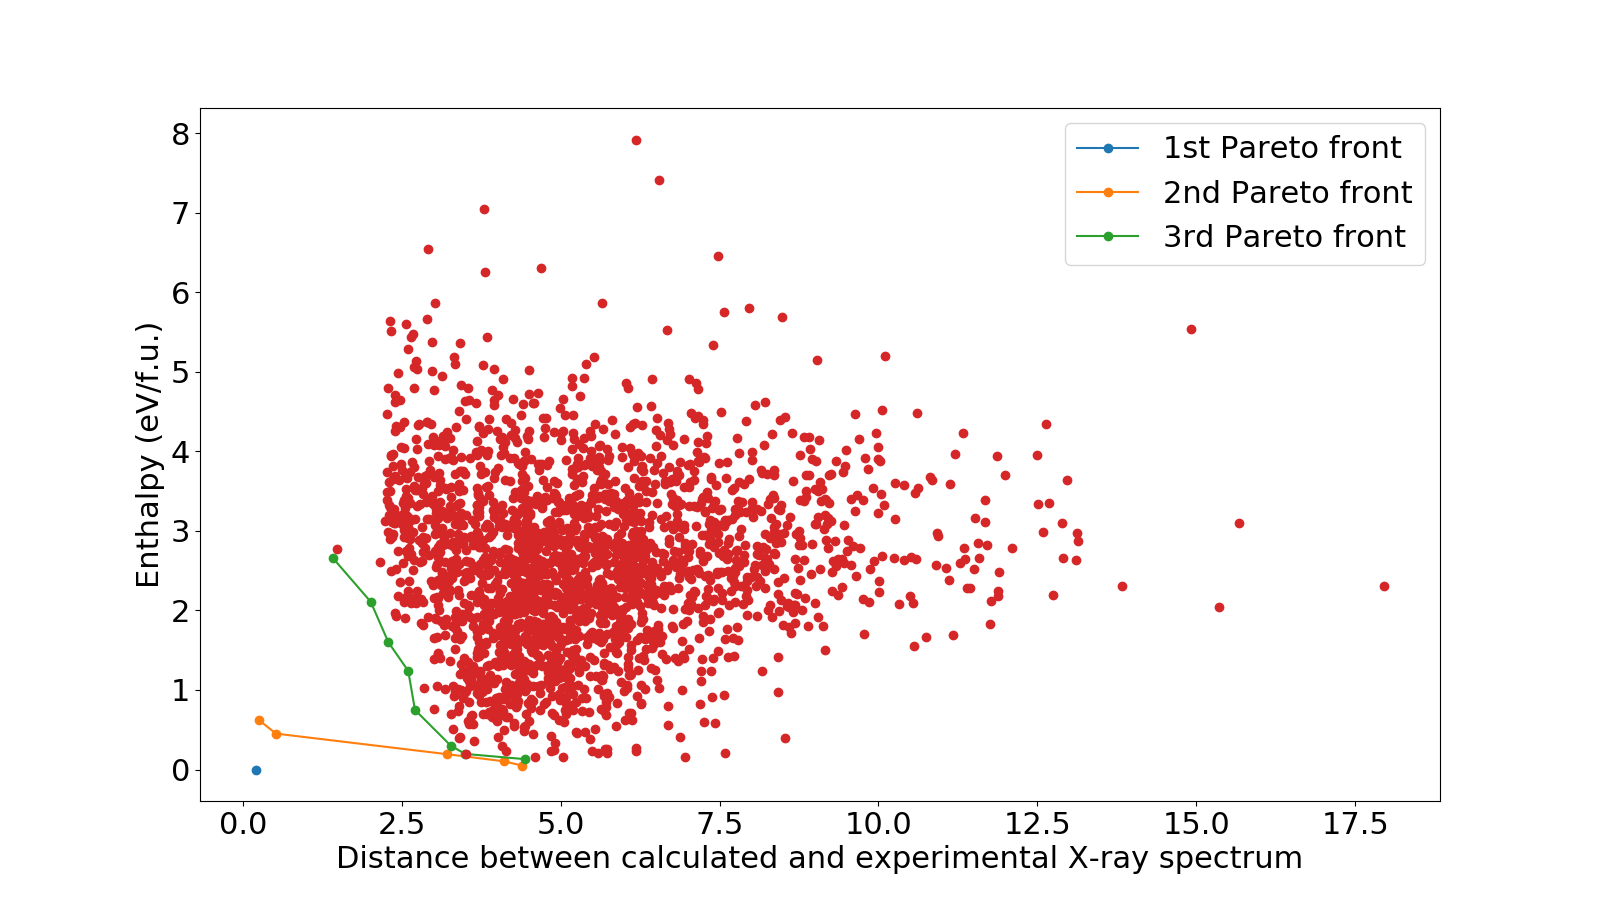
\includegraphics[width=\textwidth]{pareto.png}
	\caption{Graph produced by the script \texttt{pareto\_picture.png} from the results of an USPEX run in which stability of the system \ch{K4Ta4W4O24} has been optimized together with the agreement with an experimental powder XRD spectrum.}
	\label{fig:pfronts}
\end{figure}
\begin{figure}
	\centering
	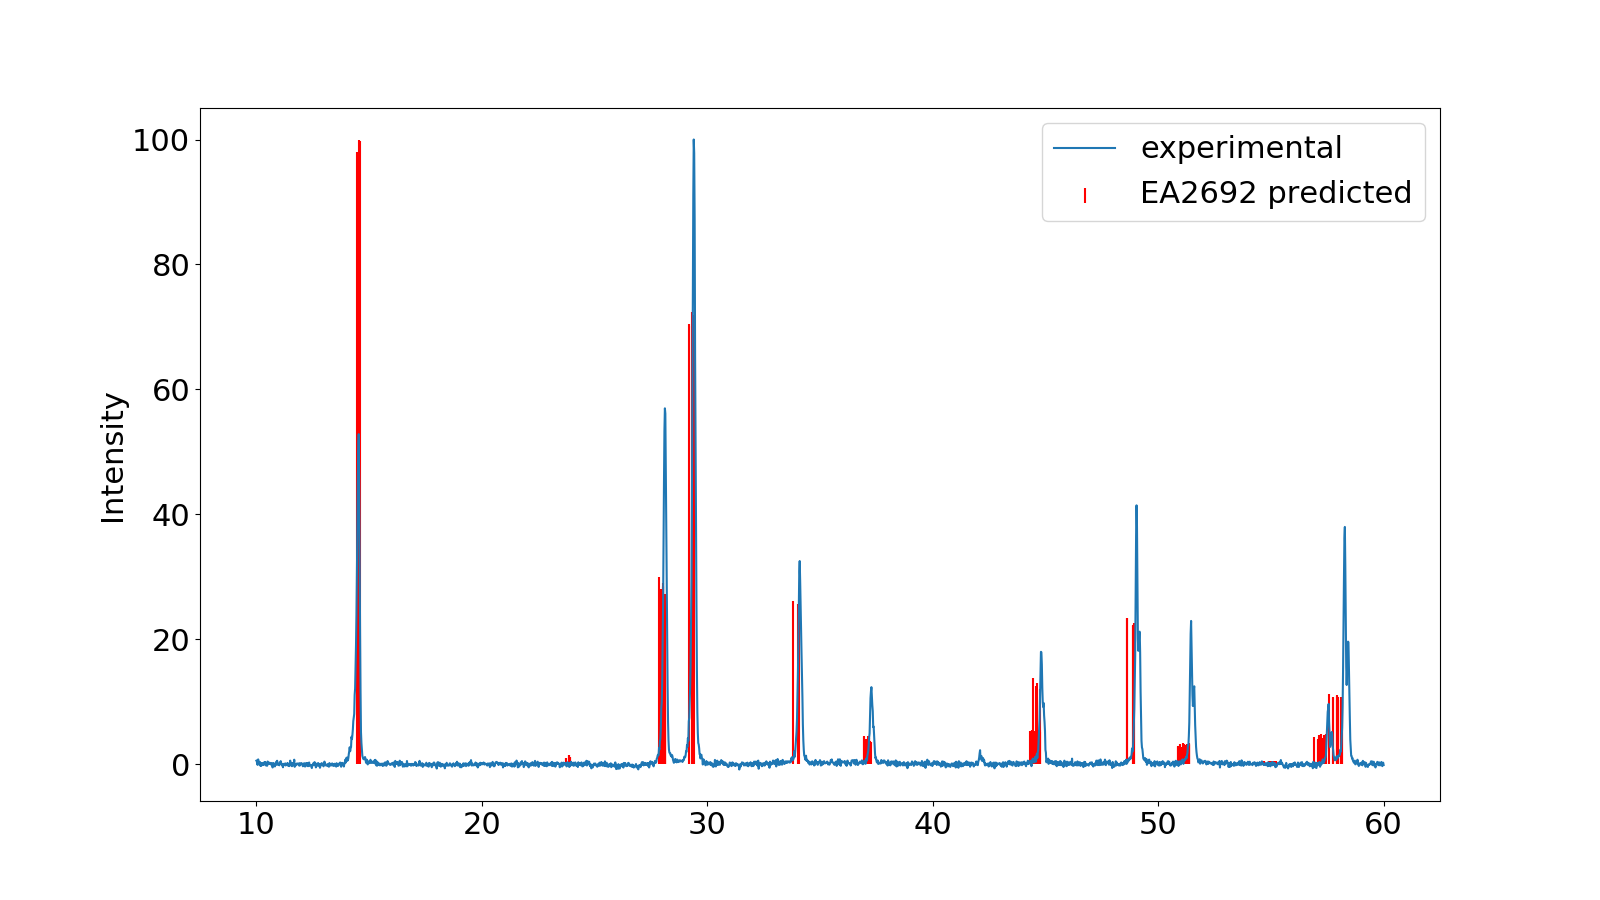
\includegraphics[width=\textwidth]{1_0.210_0.000_EA2692.png}
	\caption{Graph produced by the script \texttt{pareto\_picture.png} from the results of an USPEX run in which stability of the system \ch{K4Ta4W4O24} has been optimized together with the agreement with an experimental powder XRD spectrum.}
	\label{fig:comparison}
\end{figure}
The name of these files have the format \texttt{rank\_F\_enthalpy\_ID}, where:
\begin{description}
	\item[rank] is the progressive number of the Pareto front
	\item[F] is the agreement F between simulated and given spectra
	\item[enthalpy] is the enthalpy of the structure
	\item[ID] is the structure ID from the USPEX run
\end{description}
\textbf{Example}: \texttt{python pareto\_picture.py}

\section{single\_plot.py}

This simple script is used to obtain a plot of the predicted powder XRD spectrum of a single structure against the experimental spectrum. It takes in input, at lines 12-14, the following three parameters:
\begin{enumerate}
	\item the wavelength of the incident radiation in \SI{}{\angstrom}
	\item the name of the file containing the geometry of the structure in POSCAR format
	\item the name of the file containing the experimental spectrum
\end{enumerate}
\textbf{Example}: \texttt{python single\_plot.py}

\section{scxrd\_screening}

This script performs a screening of USPEX results, looking for the structures that best match an experimental single crystal X-ray spectrum. The fitness function for evaluating the agreement between theoretical and experimental spectra is the weighted R-factor (see appendix \ref{sec:scspectracomp}). Notice that the USPEX run must have been performed at fixed cell parameters. The script contains the following input parameters:
\begin{enumerate}
	\item the name of the \texttt{gatheredPOSCARS} file from the USPEX run
	\item the name of the HKL file containing experimental reflections
\end{enumerate}
The script outputs a file \texttt{results.txt} which contains a list of ordered structure IDs with their relative weighted R-factor, from the most fit to the least fit.

\vspace{0.2cm}
\noindent \textbf{Example}: \texttt{python scxrd\_screening.py}

\appendix
\appendixpage

\section{Powder spectra comparison}
\label{sec:powderspectracomp}

We developed a code which computes, from the experimental powder XRD spectrum and the USPEX output, the degree of disagreement (fitness) of each relaxed structure with the experimental data. The USPEX calculation and the experimental spectrum do not need to be exactly at the same pressure, but the two pressures need to be \emph{close}, that is, no more than \SI{20}{GPa} apart.

Since we have a pressure difference, we first translate each calculated structure to the experimental pressure by using the Birch-Murnaghan equation
\begin{equation*}
	\Delta P = \frac{3 B_0}{2} \left[ \left( \frac{V_0}{V} \right)^{\frac{7}{3}} - \left( \frac{V_0}{V} \right)^{\frac{5}{3}} \right] \left\{ 1 + \frac{3}{4} \left( B'_0 - 4 \right) \left[ \left( \frac{V_0}{V} \right)^{\frac{2}{3}} - 1 \right] \right\}
\end{equation*}
where $\Delta P$ is the pressure difference, $V_0$ is the volume of the unit cell at the calculated pressure, $V$ is the volume at the experimental pressure, $B_0$ is the bulk modulus and $B'_0$ is the derivative of the bulk modulus with respect to pressure. For $B_0$ and $B'_0$ we take the average values $B_0 = 300$ and $B'_0 = 3$. 

Assuming that, for small pressure variations, also $V_0/V$ will be small, we approximate the Birch-Murnaghan equation to a second order Taylor expansion in $V_0/V$ and we get the volume $V$ at the experimental pressure:
\begin{equation*}
	V = \frac{300}{150 + \sqrt{22500 + 300 \Delta P}} V_0
\end{equation*}
Then we define the following scaling factor
\begin{equation*}
	k = \sqrt[3]{\frac{300}{150 + \sqrt{22500 + 300 \Delta P}}}
\end{equation*}
that will be used to rescale the lattice parameters of all the calculated structures. After this rescaling, the relaxed structures are symmetrized with a tolerance of 0.2 \SI{}{\angstrom} and the theoretical XRD spectra are computed. Both the theoretical and the experimental spectra are in the form of a series of peaks.

In the case of powder XRD spectra, for each peak we know the diffraction angle and the relative intensity, while the intensity of the highest peak in each spectrum has been conventionally given the value 100. We define a \emph{match} between a theoretical and an experimental peak the case when the two peaks are less than \emph{match\_tol} degrees apart, regardless of their intensities. The fitness between a calculated powder XRD spectrum and the experimental spectrum is defined by the following fitness function
\begin{equation*}
	F = \sum_{i, j}^{match} \left( \frac{h_i^{exp} - h_j^{th}}{100} \right)^2 \left( \frac{h_i^{exp}}{100} \right)^2 + \sum_i^{exp \, rest} \left( \frac{h_i^{exp}}{100} \right)^2 + \sum_i^{th \, rest} \left( \frac{h_i^{th}}{100} \right)^2
\end{equation*}
where the $h_i$ are diffraction intensities. The first term of the fitness is a sum over the matched peaks, and each addend of this sum will be smaller the more the intensities of the two matched peaks are close to each other. The second term is a sum over the experimental peaks that are left after our matching, we call these peaks \emph{experimental rest}. The third term, analogously, is a sum over the \emph{theoretical rest}. It is clear that a low value of F gives a good agreement between calculated and experimental powder XRD spectra, allowing a quick identification of promising candidates in the USPEX output.

\section{Single crystal spectra comparison}
\label{sec:scspectracomp}

In the case of single crystal XRD spectra, for each reflection we know the Miller indices $(h, k, l)$, its intensity $I$ and its uncertainty of measure $\sigma$. As fitness we use the weighted R-factor, given by
\[
	wR = \sqrt{\frac{\sum \frac{1}{\sigma^2} (I_{exp} - I_{th})^2}{\sum \frac{1}{\sigma^2} I_{exp}^2}}
\]
where the sums run over all the experimental reflections and theoretical reflections at the same Miller indices $(h, k, l)$. If an experimental reflection is not matched by any theoretical reflection an error is returned, while in the opposite case the unmatched theoretical reflection is simply ignored.

\end{document}